\chapter{Introduction to exponential integration methods}

\begin{tcolorbox}[title=Résumé du chapitre : Introduction aux méthodes d'intégration exponentielles, colframe=black!50!white]
  \paragraph{}
  Le but de ce chapitre est de d'introduire un nouveau type de méthodes d'intégration temporelle.

  \paragraph{}
  Les méthodes classiquement utilisées dans la résolution des problèmes stationnaires sont souvent réutilisées après être adaptées dans la résolution de problèmes instationnaires intégrés avec de grands pas de temps pour s'affranchir des critères de stabilité de l'intégration explicite.
  Nous présentons dans ce chapitre le principe des méthodes d'intégration exponentielles, qui sortent de la dichotomie explicite/implicite.
  Nous décrivons ensuite plus en détail la famille des méthodes Rosenbrock exponentielles, qui seront utilisées par la suite.
  Nous réalisons également une brève analyse théorique de ces méthodes.

  \paragraph{}
  Comme leur nom l'indique, ces méthodes reposent sur l'exponentielle.
  Leur difficulté vient du fait qu'elles nécessitent de calculer des exponentielles de matrices, de très grande taille dans nos applications.
  Nous détaillons donc comment ce calcul est réalisé en utilisant des sous-espaces de Krylov.

  \paragraph{}
  Finalement, nous essayons une méthode exponentielle développée dans CEDRE sur un cas analytique simple.
  Nous montrons alors la pertinence de cette nouvelle méthode au vu de ses performances sur ce cas.
\end{tcolorbox}


  \vspace{1cm}
  \paragraph{}
  In this thesis, we were interested in finding solutions to steady problems.
  As we explained in the previous part, we use implicit time integration methods to efficiently get solutions to such problems.
  This is a pretty standard choice: most computational fluid dynamics solvers use implicit time integration methods to solve steady problems.
  The reason is that they can use larger time steps than their explicit counterparts.
  Because of this advantage, they are also often used when solving unsteady problems but with large time steps.
  Indeed, solving an unsteady problem with large time steps is similar to solving a steady problem.
  Most of what is done towards solving the steady problem can therefore be reused for unsteady problems with large time steps.

  \paragraph{}
  Even if implicit time integration methods are quite standard when solving problems with large time steps, there are other less conventional methods we could choose from.
  We could step out from the explicit implicit dichotomy, and decide to use IMplicit-EXplicit, or IMEX, methods.
  They split the function from the ordinary differential equation (\ref{eq:ode}) into two parts: the stiff part that is integrated by an implicit method, because of its stiffness, and the other part that can just be integrated with an explicit method.
  The Additive Semi-Implicit Runge--Kutta methods, or ASIRK methods, are such methods \cite{Zhong1996}.
  They are already in use in computational fluid dynamics problems, such as fluid-structure interaction problems \cite{HuangPerssonZahr2019}.
  Previous work already implemented ASIRK methods in our solver CEDRE for specific multiphysics applications.
  Some methods are even less common and correspond to a total paradigm shift: the parallel time integration methods \cite{Nievergelt1964, LionsMadayTurinici2001}.
  Just as we classically split the computational domain over processes and compute the spatial discretisation method in parallel, parallel time integration methods decompose the time integration interval into subintervals.
  They then solve the ordinary differential equation on each interval concurrently then ensure the continuity between the subintervals.
  They then iterate with Newton's method to find the solution over the whole time integration interval.
  As a result, they can approximate accurately the solution at a later time without knowing accurately the solution at a previous time.
  Despite being nontraditional, they were successfully used to solve fluid-structure interaction problems or Navier--Stokes problems \cite{GanderVandewalle2007}.
  They were even more recently used to solve simple turbulent flow problems \cite{Lunet2018}.
  They can even be used in a more convoluted way, with for instance exponential methods \cite{GanderGuettel2013}.
  Just as parallel time integration is inspired by parallel spatial discretisation, some other time integration methods are inspired by spectral discretisation methods.
  Time spectral methods, that were originally used for fluid dynamic time-periodic problems \cite{GopinathJameson2005, GopinathJameson2006}, are now used on non-periodic problems \cite{EkiciDjeddiLiEtAl2020}.
  But as both time parallel integration methods and time spectral methods are considered highly unconventional they require a major refactoring of the solver, which should be avoided for large-scale industrial solvers.
  In this part, however, we prefer to focus on another class of time integration methods.


  \section{Exponential integration methods}

    \paragraph{}
    Let us focus on methods known as exponential methods.
    Despite being known for a long time \cite{Pope1963}, they were not widely used in computational fluid dynamics, because of some difficulties that are explained later, but still interested some scientists \cite{EdwardsTuckermanFriesnerEtAl1994}.
    They started to come back in the literature \cite{HochbruckOstermann2005, HochbruckOstermann2010} and are now being used on applications similar to ours \cite{NieZhangZhao2006, BhattKhaliqWade2018}.

    \paragraph{}
    The ordinary differential equation
    \begin{equation}\label{eq:ode_2}
      \frac{\mathrm{d} y}{\mathrm{d} t} = f\left(y\right)
    \end{equation}
    is the same as the ordinary differential equation (\ref{eq:ode}) from the previous part but with different notations.
    The main idea of exponential integration methods is to start from the ordinary differential equation (\ref{eq:ode_2}) and split the function $f$ into a linear part and a nonlinear part:
    \begin{equation}\label{eq:ode_split}
      \frac{\mathrm{d} y}{\mathrm{d} t} = Ly + N\left(y\right) .
    \end{equation}
    This decomposition is sometimes natural for some particular equations, but in the more general case it is always possible: it consists in choosing a linear part $L$ and then setting the nonlinear part $N\left(y\right) = f(y) - Ly$.
    There are then an infinite number of decompositions, but we will see later that some are more interesting.

    \paragraph{}
    To define the time integration step, we start from the current estimate of the solution $y_n$ that we assume to be exact: $y_n = y\left(t_n\right)$.
    We note $\Delta t = t_{n+1} - t_n$ as we work here with a fixed $n$.
    We can integrate equation (\ref{eq:ode_2}) using the variation of constants formula to get:
    \begin{equation}\label{eq:ode_int}
      y\left(t_{n+1}\right) = e^{\Delta t L} y_n + \int_{t_n}^{t_{n+1}} e^{\left(t_{n+1} - t\right) L} N\left(y\left(t\right)\right) \mathrm{d}t .
    \end{equation}
    The exponential integration methods then approximate the integral to compute the next value $y_{n+1}$.
    What defines the method is how it approximates this integral.
    As we can see in equation (\ref{eq:ode_int}), the linear part is treated exactly and the nonlinear one is approximated.
    If there is no nonlinear part, with $N = 0$, then the solution $y_{n+1}$ is exact.
    If there is no linear part, with $L = 0$, then equation (\ref{eq:ode_int}) transforms into
    \begin{equation}\label{eq:ode_int_classic}
      y\left(t_{n+1}\right) = y_n + \int_{t_n}^{t_{n+1}} N\left(y\left(t\right)\right) \mathrm{d}t
    \end{equation}
    and the exponential integration method behaves like a standard time integration method.
    This is the advantage of exponential integration methods: at best they are exact methods, and at worst, they are equivalent to traditional methods.

    \paragraph{}
    Similarly to classic methods, there are explicit \cite{BhattKhaliqWade2018} and implicit \cite{NieZhangZhao2006} exponential integration methods.
    It depends on whether it uses $y_{n+1}$ or not to compute the integral from equation (\ref{eq:ode_int}).

    \paragraph{}
    Before continuing, let us define some functions that are going to be convenient later on.
    Let the functions $\varphi_k$ be defined by:
    \begin{equation}
      \left\{\begin{aligned}
        \varphi_0 &: z \mapsto e^z \\
        \forall k \in \mathbb{N}^*, \varphi_{k} &: z \mapsto \int_0^1 e^{\left(1 - \theta\right)z} \frac{\theta^{k-1}}{\left(k-1\right)!} \mathrm{d}\theta .
      \end{aligned}\right.
    \end{equation}
    They could also be defined using the recurrence relation:
    \begin{equation}
      \left\{\begin{aligned}
        \varphi_0 &: z \mapsto e^z \\
        \forall k \in \mathbb{N}, \varphi_{k+1} &: z \mapsto \frac{\varphi_k\left(z\right) - \varphi_k\left(0\right)}{z} ,
      \end{aligned}\right.
    \end{equation}
    or directly using their analytic formula:
    \begin{equation}
      \forall k \in \mathbb{N}, \varphi_{k} : z \mapsto \sum_{i = 0}^{+\infty} \frac{z^i}{\left(i + k\right)!} .
    \end{equation}
    This analytic formula ensures it is well-defined for squared matrices.


  \pagebreak
  \section{Exponential Rosenbrock--Euler method}

    \subsection{Definition of the exponential Rosenbrock--Euler method}

      \paragraph{}
      The exponential Euler method is the most basic one, and it can be used to understand exponential integration methods.
      Just as the Euler method assumes that $N\left(y\right)$ is constant and equal to $N\left(y_n\right)$ in equation (\ref{eq:ode_int_classic}), its exponential counterpart makes the same assumption but in equation (\ref{eq:ode_int}).
      It then gives:
      \begin{equation}
        y_{n+1} = e^{\Delta t L} y_n + \Delta t \varphi_1\left(\Delta t L\right) N\left(y_n\right)
      \end{equation}
      using the $\varphi_1$ function defined above, and finally:
      \begin{equation}\label{eq:expeuler}
        y_{n+1} = y_n + \Delta t \varphi_1\left(\Delta t L\right) f\left(y_n\right) .
      \end{equation}
      Note the difference with the corresponding standard Euler method, for which the $\varphi_1$ function is replaced with the identity function.
      If there is no linear part in the decomposition, with $L = 0$, then nothing is treated differently by the exponential method, and the standard explicit Euler method is recovered.

      \paragraph{}
      In this method, the linearisation $L = f'\left(y_n\right)$ is assumed.
      Because of this choice, the method is called the exponential Rosenbrock--Euler method.
      We will discuss the nomenclature below.
      This choice feels natural and minimises the error of the method as is shown in the following.
      This choice is frequent among exponential integration methods, despite some methods using a fixed linearisation $L = f'\left(y_0\right)$.
      The difference is that a new Jacobian matrix is required at each iteration of the time integration method, but it is something we are used to with our traditional implicit methods.
      It is worth noting that we might want to try the implicit equivalent of this method by taking $N\left(y\right) = N\left(y_{n+1}\right)$ in equation (\ref{eq:ode_int}).
      However, because we took $L = f'\left(y_n\right)$, $N'\left(y\right) = 0$ and after a linearisation the two variants are equivalent.


    \subsection{Analysis of the exponential Rosenbrock--Euler method}

      \paragraph{}
      From the definition of the method and equation (\ref{eq:ode_int}), we have that the error made after one step is:
      \begin{equation}
        \begin{aligned}
          y\left(t_{n+1}\right) - y_{n+1} &= \int_{t_n}^{t_{n+1}} e^{\left(t_{n+1} - t\right) L} N\left(y\left(t\right)\right) \mathrm{d}t  - \Delta t \varphi_1\left(\Delta t L\right) N\left(y_n\right) \\
          &= \int_{t_n}^{t_{n+1}} e^{\left(t_{n+1} - t\right) L} \left( N\left(y\left(t\right)\right) - N\left(y_n\right) \right)
        \end{aligned}
      \end{equation}
      We take the Taylor series of the nonlinear part:
      \begin{equation}
        N\left(y\right) = \sum_{i = 0}^{+\infty} \frac{N^{\left(i\right)}\left(y_n\right)}{i!}\left(y - y_n\right)^i
      \end{equation}
      and in particular, using the fact that
      \begin{equation}
        \begin{aligned}
          y\left(t\right) &= y_n + y'\left(t_n\right)\left(t - t_n\right) + O\left(\left(t - t_n\right)^2\right) \\
          & = y_n + f\left(y_n\right)\left(t - t_n\right) + O\left(\left(t - t_n\right)^2\right)
        \end{aligned}
      \end{equation}
      the partial series of order 2 is:
      \begin{equation}
        N\left(y\left(t\right)\right) = N\left(y_n\right) + N'\left(y_n\right)f\left(y_n\right)\left(t - t_n\right) + O\left(\left(t - t_n\right)^2\right) .
      \end{equation}
      The error of the method is then:
      \begin{equation}
        \begin{aligned}
          y\left(t_{n+1}\right) - y_{n+1} &= \int_{t_n}^{t_{n+1}} e^{\left(t_{n+1} - t\right) L} \left( N'\left(y_n\right)f\left(y_n\right)\left(t - t_n\right) + O\left(\left(t - t_n\right)^2\right) \right) \mathrm{d}t \\
          &= \Delta t^2\varphi_2\left(\Delta t L\right) N'\left(y_n\right)f\left(y_n\right) + O\left(\Delta t^3\right) .
        \end{aligned}
      \end{equation}
      The decomposition chosen earlier is now justified: if $L = f'\left(y_n\right)$ and therefore $N'\left(y_n\right) = 0$ then $y\left(t_{n+1}\right) - y_{n+1} = O\left(\Delta t^3\right)$ and the method is of order 2.
      This is a noticeable property of this method: despite being a single-step method it has a second-order of accuracy.
      A more rigorous analysis can be found in \cite{HochbruckOstermannSchweitzer2009}.

      \paragraph{}
      It is much harder to analyse the stability of this method, and more generally of exponential methods.
      Indeed, the stability analysis is done on the Dahlquist test equation (\ref{eq:dahlquist}).
      But as this equation is linear, exponential methods can solve them exactly no matter the time step size.
      We can still write the single step equation (\ref{eq:single_step}) $y_{n+1} = g\left(\Delta tJ\right)y_n$ with $g\left(z\right) = e^z$, and get the corresponding stability region which is the left half complex plane.
      We could then conclude that the method is A-stable.
      The issue with exponential methods is that the standard stability analysis is no longer pertinent.
      We tried to do a better stability analysis for simple exponential methods such as the exponential Rosenbrock--Euler method, but we did not succeed.
      Some work in the literature does define some stability notions for exponential methods \cite{DuZhu2004}, but usually takes a linear $N$.
      It goes against the idea that all the linear part of $f$ is in $L$ and $N$ is purely nonlinear.
      We did not find a stability analysis that was satisfying to us.


  \section{Exponential Runge--Kutta and Rosenbrock methods}

    \paragraph{}
    When we introduced explicit methods, we used more convoluted approximations than the explicit Euler methods for the integral in equation (\ref{eq:ode_int_classic}).
    This gave the Runge--Kutta methods.
    The same can be done for the integral in equation (\ref{eq:ode_int}) to get exponential Runge--Kutta methods.
    The difference with a standard Runge--Kutta method is that the quadrature coefficients are now functions of the matrix $L$:
    \begin{equation}
      \left\{\begin{aligned}
        y_{n+1} &= e^{\Delta t L} y_n + \Delta t \sum_{i = 1}^k b_i\left(\Delta t L\right) N\left(y_{n,i}\right) \\
        \textrm{with}\quad y_{n,i} &= e^{c_i \Delta t L} y_n + \Delta t \sum_{j = 1}^{i-1} a_{ij}\left(\Delta t L\right) N\left(y_{n,j}\right) .
      \end{aligned}\right.
    \end{equation}
    The Butcher tableau that we used to represent the Runge--Kutta methods is also used to represent the exponential Runge--Kutta methods.
    For instance, the Butcher tableau of the exponential Rosenbrock--Euler method, which is a special simple case of exponential Runge--Kutta methods, is shown in table \ref{tab:exprb_butcher}.

    \paragraph{}
    Until now, we have not been exact when naming the methods we constructed here.
    From the literature, exponential Runge--Kutta methods are defined just as we did above, except they use a fixed linearisation: $L = f'\left(y_0\right)$ \cite{HochbruckOstermann2005}.
    It is because they were developed for semilinear parabolic problems:
    \begin{equation}
      \frac{\mathrm{d} y}{\mathrm{d} t} + Ay = r\left(y\right) .
    \end{equation}
    They are used when the remainder $r$ is small or at least bounded in terms of $A$.
    This is not the case in our applications, and in many others so that is why another type of exponential method was introduced: exponential Rosenbrock methods \cite{HochbruckOstermannSchweitzer2006}.
    They can be seen as a variation of the exponential Runge--Kutta methods where the linearisation is done at each time step.
    The issue is that a new Jacobian matrix is needed at each iteration, but once again we are used to this with implicit methods.

    \paragraph{}
    The nomenclature is a bit blurry to us, as the distinction between exponential Runge--Kutta and exponential Rosenbrock methods is not the same as the one between Runge--Kutta methods and Rosenbrock methods.
    First of all, the exponential Rosenbrock method is not implicit contrary to its standard counterpart.
    Furthermore, it would make sense to us to name an exponential integration method base on the underlying method used to approximate the integral from equation (\ref{eq:ode_int}), and exponential Rosenbrock methods do not use Rosenbrock methods to do it.
    The only parallel we found was that the Rosenbrock methods do a linearisation at each inner stage, and the exponential Rosenbrock methods do a linearisation at each step of the time integration.
    It just seems that in the literature, the term \emph{Rosenbrock} indicates that the linearisation is computed at each step instead of once at the beginning, with no apparent link with Rosenbrock methods.

    \paragraph{}
    Just as the Runge--Kutta method has order conditions for its quadrature coefficients, the exponential Rosenbrock method quadrature functions must follow some rules to ensure the expected order.
    To be consistent, it must have:
    \begin{equation}
      \sum_{i = 1}^k b_i = \varphi_1 .
    \end{equation}
    It is reasonable to want multiple-stage methods to have a higher order than the single-stage exponential Euler method, and therefore it must also have
    \begin{equation}
       \sum_{j = 1}^{i-1} a_{ij} = z \mapsto c_i \varphi_1\left(c_i z\right), \quad 1 \leq i \leq k
    \end{equation}
    to achieve a second order.
    Using these two conditions, exponential Rosenbrock methods can be written in the form:
    \begin{equation}\label{eq:exprb_defect}
      \left\{\begin{aligned}
        y_{n+1} &= y_n  + \Delta t \varphi_1\left(\Delta t L\right) f\left(y_n\right) + \Delta t \sum_{i = 2}^k b_i\left(\Delta t L\right) D_{n,i} \\
        \textrm{with}\quad y_{n,i} &= y_n  + c_i \Delta t \varphi_1\left(c_i \Delta t L\right) f\left(y_n\right) + \Delta t \sum_{j = 2}^{i-1} a_{ij}\left(\Delta t L\right) D_{n,j}
      \end{aligned}\right.
    \end{equation}
    using $D_{n,i} = N\left(y_{n,i}\right) - N\left(y_n\right)$.
    This form shows that exponential Rosenbrock methods are variations of the exponential Euler method.
    The defects $D_{n, i}$ are small in size, so less computational effort can be spent when computing their contribution.

    \paragraph{}
    Among exponential Rosenbrock methods, we looked at the ExpRB32 method from \cite{HochbruckOstermannSchweitzer2009} and ExpRB42 methods from \cite{Luan2017}.
    They were developed as adaptive methods, but we will use them without the error estimate as standard methods.
    They are both 2-stage exponential Rosenbrock methods and achieve respectively a third and fourth order of accuracy.
    This shows the quality of exponential Rosenbrock methods.
    Their Butcher tableaux are in table \ref{tab:exprb_butcher}.
    For both methods, the most complex coefficient is $b_1$, however equation (\ref{eq:exprb_defect}) tells us that it will not be computed.
    We decided to work with those two methods, along with the Rosenbrock--Euler method, as they are simple among exponential methods and are supposedly well suited for our problems.
    They give us methods with orders of accuracy from 2 to 4.
    But what is interesting to us is that on linear problems those methods are exact, or with an infinite order of accuracy.
    As our problems are not purely linear, it means that the linear part will be solved exactly while the nonlinear part will be solved with a still good order of accuracy.

    \begin{table}
      \center
      \begin{tabular}{M{.25\textwidth}M{.3\textwidth}M{.3\textwidth}c}
        \begin{tabular}{c|c}
          \multicolumn{1}{c}{} \\ 0 \RKBar $\varphi_1$
        \end{tabular} &
        \begin{tabular}{c|cc}
          0 \\ 1 & $\varphi_1$ \RKBar $\varphi_1 - 2 \varphi_3$ & $2\varphi_3$
        \end{tabular} &
        \begin{tabular}{c|cccc}
          0 \\ $\frac{3}{4}$ & $\frac{3}{4}\varphi_1\left(\frac{3}{4} \cdot\right)$ \RKBar $\varphi_1 - \frac{32}{9} \varphi_3$ & $\frac{32}{9}\varphi_3$
        \end{tabular} & \\[20pt]
        Exponential Rosenbrock--Euler & ExpRB32 & ExpRB42 \\
      \end{tabular}
      \caption{Butcher tableau for some exponential Rosenbrock integration methods}\label{tab:exprb_butcher}
    \end{table}


  \section{Evaluating matrix functions}

    \paragraph{}
    At first glance, exponential methods may seem too good to be true.
    Indeed, they give explicit methods with few stages but high order of accuracy, and they have the formidable quality that they solve exactly the linear part of the ordinary differential equation.
    In other words, the exponential Euler method should be able to get the solution of Poisson's equation after any time with a single step.
    Indeed, Poisson's equation gives often a linear ordinary differential equation after the spatial discretisation, with the Finite Volume method on a regular mesh for example.
    The exponential Rosenbrock--Euler method can solve this linear differential equation exactly, for any time step, as large as it may be.

    \paragraph{}
    The reason why exponential methods are not that good is the reason why they were not used for a long time after being introduced.
    It is because evaluating matrix exponential, or more generally evaluating the $\varphi$-functions on matrices, is not trivial.
    Indeed, the power series definition of the matrix exponential is not well suited for numerical evaluations.
    In particular, in our context, computing the powers of the matrix is completely out of the question.
    The dimension of our matrices can get large, and the powers of the matrices would lose the sparsity.
    In fact, any approximation working directly with the matrix would not be satisfying.
    The question of how to evaluate $\varphi$-functions in the context of exponential methods is a subject of active research, as in this extremely recent reference \cite{CaliariCassiniZivcovich2023}. 
    We will however use more standard well-established algorithms.

    \paragraph{}
    The other issue with exponential methods is the question of the Jacobian matrix.
    Exponential Runge--Kutta reuse the same matrix throughout the computation but it is not a good idea in our applications since the nonlinear part can change.
    Exponential Rosenbrock methods were introduced for this reason but they require the computation of a new Jacobian matrix at each iteration.


    \subsection{Evaluating matrix functions with Krylov subspace methods}

      \paragraph{}
      The solution for both issues is the same: Krylov subspace methods.
      The Cayley--Hamilton theorem ensure that the exponential of a matrix is a polynomial of degree less or equal to $N$ where $N$ is the dimension of the matrix.
      Instead of looking for the matrix exponential as an infinite series, we can look for an $N$-order polynomial.
      Moreover, exponential methods do not need to evaluate the exponential or the $\varphi$-functions of the matrix, but their effect when applied to a vector.
      For instance, the exponential Rosenbrock--Euler method from equation (\ref{eq:expeuler}) does not need to compute $\varphi_1\left(\Delta t L\right)$ but $\varphi_1\left(\Delta t L\right)f\left(y_n\right)$.
      It means we do not need to evaluate a given function $h$ on the matrix $A$, but to compute the effect of $h\left(A\right)$ on the vector $b$.
      For exponential methods, $h$ is a linear combination of $\varphi$-functions, and is therefore analytic.
      The idea, originally developed to approximate eigenvalues of a large sparse matrix, is to use a Krylov subspace method to approximate $h\left(A\right)b$ \cite{Saad1992, Sidje1998}.
      In fact, it is similar to using a Krylov subspace method to solve the linear system $Ax = b$: it means taking $h = z \mapsto z^{-1}$.
      The Krylov subspace method produces with the Arnoldi iteration the relation, at the $m$-th iteration:
      \begin{equation}\label{eq:arnoldi}
        AV_m = V_{m+1} \tilde{H}_m = V_m H_m + h_{m+1, m} v_{m+1} e_m^T .
      \end{equation}
      The columns of $V_m$, $v_1, \dots, v_m$, form an orthonormal basis of the Krylov subspace:
      \begin{equation}
        \krylov[A, b]{m} = \operatorname{Vect}\left( b, Ab, \dots, A^{m-1}b \right)
      \end{equation}
      with $v_1 = b / \norm[2]{b}$.
      The matrix $\tilde{H}_m$ is a Hessenberg matrix and $H_m$ is the square matrix equal to $\tilde{H}_m$ without its last line:
      \begin{equation}
        \tilde{H}_m = \begin{pmatrix}
          h_{1,1} & h_{1,2} & \cdots    & h_{1,m} \\
          h_{2,1} & h_{2,2} & \cdots    & h_{2,m} \\
          \vdots  & \ddots  & \ddots    & \vdots  \\
          0       & \cdots  & h_{m,m-1} & h_{m,m} \\
          0       & \cdots  & 0         & h_{m+1,m}
        \end{pmatrix} , \quad H_m = \begin{pmatrix}
          h_{1,1} & h_{1,2} & \cdots    & h_{1,m} \\
          h_{2,1} & h_{2,2} & \cdots    & h_{2,m} \\
          \vdots  & \ddots  & \ddots    & \vdots  \\
          0       & \cdots  & h_{m,m-1} & h_{m,m}
        \end{pmatrix}
      \end{equation}
      The vector $v_{m+1}$ is the last column vector of $V_{m+1}$, added to the column vectors of $V_m$ to get an orthonormal basis of $\krylov[A, b]{m+1}$, and $e_m$ is the $m$-th canonical vector $\left(0, \dots, 0, 1\right)^T$.
      Since $H_m$ represent the compression of $A$ on $\krylov[A, b]{m}$ with respect to basis $V_m$ and $b = \norm[2]{b} V_m e_1$ with $e_1 = \left(1, 0, \dots, 0\right)$, we make the approximation \cite{EiermannErnst2006}:
      \begin{equation}
        h\left(A\right)b \approx \norm[2]{b} V_m h\left(H_m\right) e_1 .
      \end{equation}

      \paragraph{}
      With this approximation, we can evaluate the function $h$ by applying it to a smaller matrix.
      We reduced the original function evaluation to the much smaller Krylov subspace.
      Since the method does not need to know the matrix but only to be able to apply it as a linear operator, we can use the matrix-free approximation (\ref{eq:matrix_free}) to approximate the Jacobian matrix $L = f'\left(y_n\right)$.
      This way, having to compute a new Jacobian matrix at each iteration of the exponential Rosenbrock method is not an issue.
      Just as Krylov subspace methods for solving linear problems, this method can be restarted to limit the size of the Krylov subspace and therefore control the memory consumption of the algorithm.
      It is even possible to define an error estimate in the approximation to dynamically control the number of iterations needed to reach a given tolerance, albeit it is more convoluted than the residual used for solving linear systems with Krylov subspace methods \cite{EiermannErnst2006}.

      \paragraph{Note:}
      Since the matrix used to evaluate the quadrature functions of the exponential Rosenbrock methods is always the same, $L$, only one Arnoldi iteration is required for one step of the method.
      This could lead to a great cost reduction, however, we did not try it in our developments.
      Indeed, our work on exponential integration methods was more to demonstrate their feasibility in our applications, but it would be interesting to use this idea for future performance enhancements.


    \subsection{Evaluating matrix exponentials}

      \paragraph{}
      With the Krylov subspace method just described, the next step is the computation of the exponential of the smaller Hessenberg matrix $H_m$.
      Attention is now paid to how to compute the exponential of relatively small dense matrices.
      Many methods use special properties of the matrices but our matrices do not share the same properties.
      Instead of using a truncated Taylor series, using the Padé approximant seems to be the best option \cite{HighamAlMohy2010}.
      The exponential function is approximated by the $\left[k/m\right]$ Padé approximant:
      \begin{equation}
        e^z \approx r_{k,m}\left(z\right) = \frac{p_{k,m}\left(z\right)}{q_{k,m}\left(z\right)} \quad\textrm{with} \left\{\begin{aligned}
          \quad p_{k,m} &= \sum_{i = 0}^k \frac{\left(k + m - i\right)! k!}{\left(k + m\right)! \left(k - i\right)!} \frac{z^i}{i!} \\
          \quad q_{k,m} &= \sum_{i = 0}^m \frac{\left(k + m - i\right)! m!}{\left(k + m\right)! \left(m - i\right)!} \frac{\left(-z\right)^i}{i!} .
        \end{aligned}\right.
      \end{equation}
      It is best to use diagonal approximants, with $k = m$, as they are more accurate \cite{HighamAlMohy2010}.

      \paragraph{}
      The final method used to compute the exponential of a dense matrix is the Scaling and Squaring method \cite{Higham2009}.
      It computes an optimal parameter $s$ and takes:
      \begin{equation}
        e^z \approx r_{m,m}\left(z/2^s\right)^{2^s} .
      \end{equation}
      The goal is to choose $s$ such as the error on the computation of the exponential is bounded, with minimal cost.
      It then decides on an optimal order $m$ for the Padé approximant.
      The matrix is scaled by $2^s$, the Padé approximant is used to compute the exponential, and the result is then squared back to the original scale.
      It is what gives its name to the method.


    \subsection{Evaluating the \texorpdfstring{$\varphi$}{phi}-functions}

      \paragraph{}
      The exponential time integration methods do not only use matrix exponential, the $\varphi_0$ function, but may use any $\varphi_k$ function.
      There is a nice relation that helps compute those functions.
      We first define the \emph{augmented} squared Hessenberg matrix:
      \begin{equation}
        \bar{H}_{m + p} = \begin{pmatrix}
          H_m & c & 0 & \cdots & 0      \\
              & 0 & 1 & \ddots & \vdots \\
              &   & 0 & \ddots & 0      \\
              &   &   & \ddots & 1      \\
          0   &   &   &        & 0
        \end{pmatrix}
      \end{equation}
      with a vector $c$ of dimension $m$.
      Then, the following relation holds \cite{Sidje1998}:
      \begingroup
      \renewcommand*{\arraystretch}{1.5}
      \begin{equation}
        \exp\left(\tau \bar{H}_{m + p}\right) = \begin{pmatrix}
          \exp\left(\tau H_m\right) & \tau \varphi_1\left(\tau H_m\right) c & \tau^2 \varphi_2\left(\tau H_m\right) c & \cdots & \tau^p \varphi_p\left(\tau H_m\right) c \\
                                    & 1                                     & \frac{\tau}{1!}                         & \ddots & \frac{\tau^{p-1}}{\left(p - 1\right)!}  \\
                                    &                                       & 1                                       & \ddots & \vdots                                  \\
                                    &                                       &                                         & \ddots & \frac{\tau}{1!}                         \\
          0                         &                                       &                                         &        & 1
        \end{pmatrix} .
      \end{equation}
      \endgroup
      The additional cost of using this augmented matrix is negligible in comparison with the cost of the rest of the methods.
      Furthermore, the methods we introduced before only need to augment with $p \leq 3$.
      By adjusting the scalar coefficient $\tau$ and reading the result in the appropriate column, we can finally compute the quadrature coefficients of our exponential Rosenbrock methods.


  \paragraph{}
  We explained how to compute one step of an exponential integration method.
  From what we have seen, the computational cost of one step of an exponential method is roughly the same as the cost of one step of an equivalent implicit method.
  For example, the computational cost of the exponential Rosenbrock--Euler method is the cost of one Jacobian matrix computation, one Arnoldi decomposition and then one function evaluation on the Hessenberg matrix.
  The implicit Euler method, which is also a one-stage method, also computes a Jacobian matrix and does an Arnoldi decomposition.
  It then inverts the Hessenberg matrix with a QR decomposition which is equivalent to applying a function to the Hessenberg matrix.
  This is why the computational costs of the implicit Euler method and the exponential Rosenbrock--Euler method are similar.

  \paragraph{}
  When we wrote the general formula for exponential Rosenbrock methods in equation (\ref{eq:exprb_defect}), we used the defects $D_{n,i}$.
  The point of this formulation is to write the exponential Rosenbrock methods as corrections of the Rosenbrock--Euler method.
  Because the defects are usually small in size, we can spend less computational power to compute their contribution to the final step.
  Practically, it means we can use smaller Krylov subspaces to account for the defects.
  It means shorter Arnoldi iterations, which means smaller Hessenberg matrices, and overall a much smaller computational cost.
  We explained why the one-stage exponential method cost is equivalent to the one-stage implicit method cost.
  Because we use the formulation (\ref{eq:exprb_defect}) and the fact that the defects are small, adding more stages to the exponential method will be less expensive than adding stages to the implicit method.


  \pagebreak
  \section{First developments in CEDRE}

    \paragraph{}
    We first tried exponential methods in the solver CEDRE.
    The development was fast as it reuses a lot of existing parts from the implicit time integration: principally the Krylov subspace methods tools.
    The matrix used in the decomposition (\ref{eq:ode_split}) can either be the traditional low-order Jacobian matrix or can use the matrix-free approximation (\ref{eq:matrix_free}).
    It shows that this work about exponential integration methods is compatible with our work about the Jacobian matrix, presented before.
    The Arnoldi decomposition (\ref{eq:arnoldi}) is computed by the same routines as the ones used for the GMRES algorithm.
    We only had to develop the Scaling and Squaring algorithm, with the computation of the Padé approximant to be able to use exponential Rosenbrock methods.
    Because it only required this development we decided to deviate from the original framework of this thesis and try this new type of time integration method.
    Now that everything was accessible, we started with the exponential Rosenbrock--Euler method, as it is the basic one.

    \paragraph{}
    To test the method, we decided to use a simple academic test case, adapted from the one proposed at the International Workshop on High Order CFD Methods (HiOCFD).
    It is a two-dimensional inviscid isentropic vortex that is convected in a periodic box.
    This vortex is a known exact solution of the unsteady Euler equations and is generally considered a good test case to analyse the accuracy of both spatial discretisation and time integration methods.
    It is a non-dimensionalised computation, and the mesh is regular over a square of length $L = 20$, with $100^2$ cells.
    The vortex is convected in a flow at a Mach number of $\operatorname{Ma} = 0.5$, with the dimensioning parameters $P_\infty = 1$ and $T_\infty = 1$.
    The undisturbed velocity is then $U_\infty \vec{e}_x$ with $U_\infty = \operatorname{Ma} \sqrt{\gamma r_\textrm{gas} T_\infty}$ and the vortex is defined using the polar coordinates system $\left(\vec{e}_r, \vec{e}_\theta\right)$:
    \begin{equation}\label{eq:covo}
      \left\{\begin{aligned}
        \vec{u} &= U_\infty \vec{e}_x + \beta U_\infty \frac{r}{R_0} e^{-r^2 / 2 R_0^2} \ \vec{e}_\theta \\[10pt]
        T &= T_\infty - \beta^2 U_\infty^2 \frac{\gamma - 1}{2 \gamma r_\textrm{gas}} e^{-r^2 / R_0^2} \\[10pt]
        P &= P_\infty \left( 1 - \frac{\beta^2 U_\infty^2}{T_\infty} \frac{\gamma - 1}{2 \gamma r_\textrm{gas}} e^{-r^2 / R_0^2} \right)^{\gamma/\left(\gamma - 1\right)} .
      \end{aligned}\right.
    \end{equation}
    The heat capacity ratio $\gamma$ is equal to $1.4$, and the specific gas constant is $r_\textrm{gas} = 1$.
    The vortex is defined by its characteristic radius $R_0 = 1$ and its intensity $\beta = 0.2$.
    This initial condition is shown in figure \ref{fig:covo_cedre_fields}.
    As we solve inviscid Navier--Stokes equations, or Euler equations, the vortex moves in the $\vec{e}_x$ direction undisturbed, and as the domain is periodic the solution after one period $\Delta T = L/U_\infty = 33.8$ is the same as the initial solution.

    \begin{figure}
      \centering
      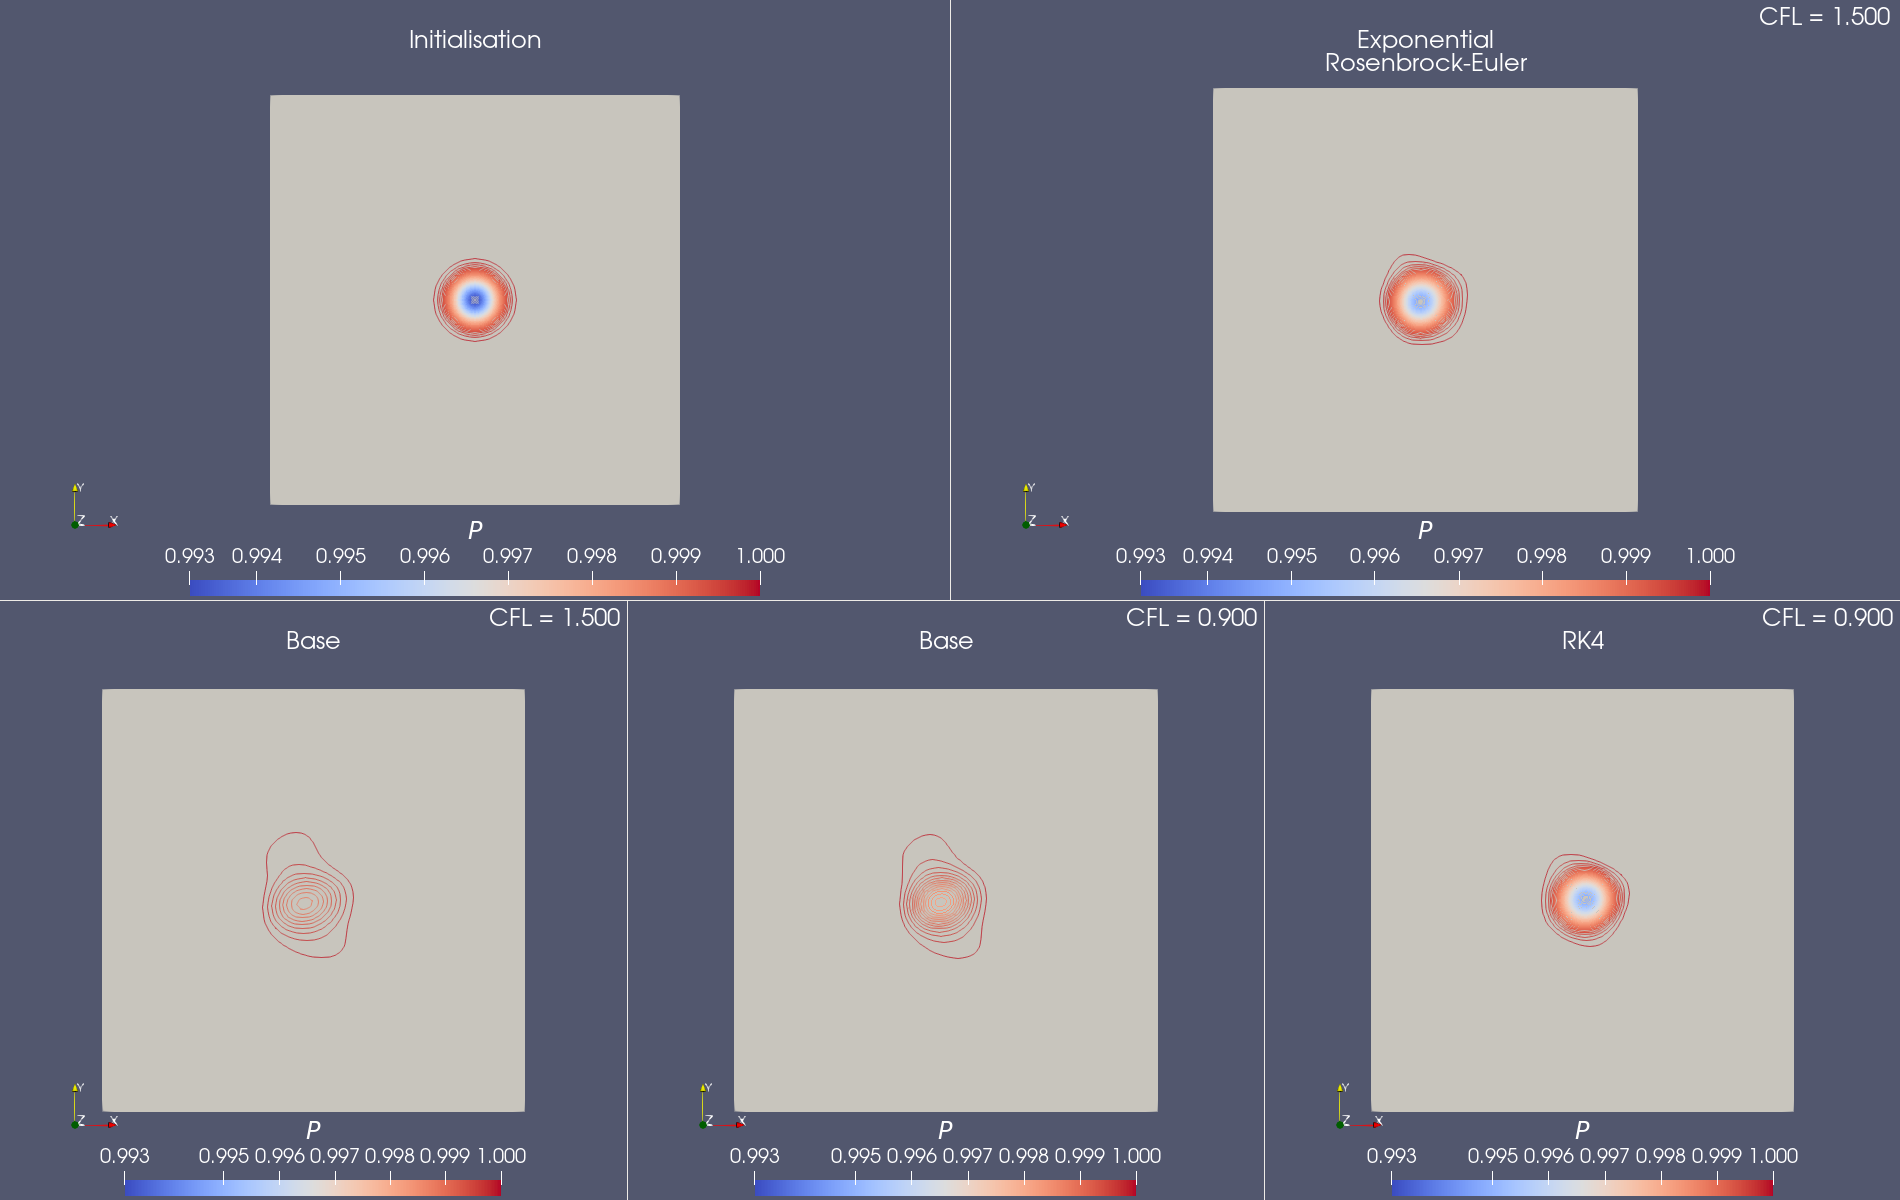
\includegraphics[width=\textwidth]{figures/covo_cedre_fields.png}
      \caption{Initial solution (top left) and solution after one period for the exponential Rosenbrock--Euler method (top right), the implicit Euler method (bottom left and center) and the explicit RK4 method (bottom right).
      The first two simulations correspond to a CFL number of $1.5$ whereas the last two to a CFL number of $0.9$.}
      \label{fig:covo_cedre_fields}
    \end{figure}

    \paragraph{}
    We compare the exponential Rosenbrock--Euler method to the standard implicit Euler method and the classic fourth-order explicit Runge--Kutta method.
    Both the implicit and the exponential methods need to compute Jacobian matrices.
    To reduce the number of variables in this comparison, both will use the traditional Jacobian matrices which is the low-order approximation.
    We then end up with two equivalent methods in terms of computational cost.
    We simulate the vortex advection throughout one period $\Delta T$.
    The solution for each method is shown in figure \ref{fig:covo_cedre_fields}.
    We first look at the bottom center and right simulations.
    We see that the explicit Runge--Kutta method preserves well enough the vortex compared to the implicit method.
    It is because the RK4 method is a fourth-order method whereas the implicit method is a first-order method.
    However, the simulations are made at a CFL number of $0.9$.
    With a higher CFL number of $1.5$, the explicit method is unstable and the computation fails.
    The implicit method is able to handle higher CFL numbers, of course as it is the reason implicit methods are used.
    But unsurprisingly we see in the bottom left figure that the solution is even worse.
    Finally, the exponential method is able to handle the higher CFL number and preserve the vortex well enough.
    It has the robustness of the implicit method and the precision of the higher-order explicit method.

    \paragraph{}
    The analysis of this simple test case is quite rudimentary.
    Indeed, we did not look finely at the error introduced by the time integration methods, but we visually compared the results.
    This work showed that at the cost of very few developments we have a method that could prove interesting for time integration with large time steps.
    Its purpose was not to precisely analyse exponential methods but to see their feasibility in our solver.
    Now that this preliminary test showed the quality of exponential time integration methods, we need to perform an actual analysis.

    \paragraph{}
    We see in figure \ref{fig:covo_cedre_fields} that even the methods that preserve the vortex, the exponential and the RK4 methods, do introduce some error.
    Indeed, the vortex after one period is not exactly the same as at the beginning, as it should be.
    We see that it loses in intensity, and the contour lines are not exactly concentric.
    Those symptoms are seen in both computations with the exponential and the higher-order explicit methods.
    Furthermore, the error in the result of those simulations looks similar.
    It is because this error does not come from the time integration method but from the spatial discretisation method.
    Indeed, the spatial discretisation method induces some error when evaluating the right-hand side of equation (\ref{eq:ode_2}).
    This error is accumulated throughout the simulation, and because of it, we could not get the exact result no matter the time integration method.
    What we can do, however, is take a spatial discretisation method such as the error it adds is small compared to the error from the time integration scheme.
    This way, the error we get at the end of the computation is mostly due to the time integration method, and it allows us to compare methods.
    Here the spatial discretisation method used in CEDRE is a second-order method.
    We need to use a higher-order spatial discretisation method to perform the analysis of exponential time integration methods.
